\documentclass[class=article, crop=false, 12pt]{standalone}
\usepackage[subpreambles=true]{standalone}
\usepackage{../.common/common}


\author{Tony Shing}
%\pretitle{Supplementary}

\topic{T10B (Thermodynamics)}
\title{Maxwell-Boltzmann Distribution}

\version{2025} % leave blank for omitting

\begin{document}

\maketitle


\begin{overview}
    \begin{itemize}
        \item Prerequisite: Probability, extending to continuous random variables
        \item Thermal fluctuation and Boltzmann factor
        \item Maxwell-Boltzmann distribution, average speed of ideal gas
    \end{itemize}

\end{overview}


% content begins here
% Section %%%%%%%%%%%%%%%%%%%%%%%%%%%%%%%%%%%%%%%%%%%%%%%%%%%%
\section{Probability Distribution: Discrete \& Continuous}

%%%%%%%%%%%%%%
\subsection{Probabilty Mass Function (PMF)}

For random variables that can be picken from a finite number cases,
we describe them using the \bf{probability mass function} (PMF), $P(x)$,
or most of the time we just call them probabilities.\\

E.g. By throwing 2 dices and sum their values, 
we obtain a list of different probabilities for getting any integer between 2 to 12.

\begin{center}
    \begin{minipage}{0.55\linewidth}
        \centering
        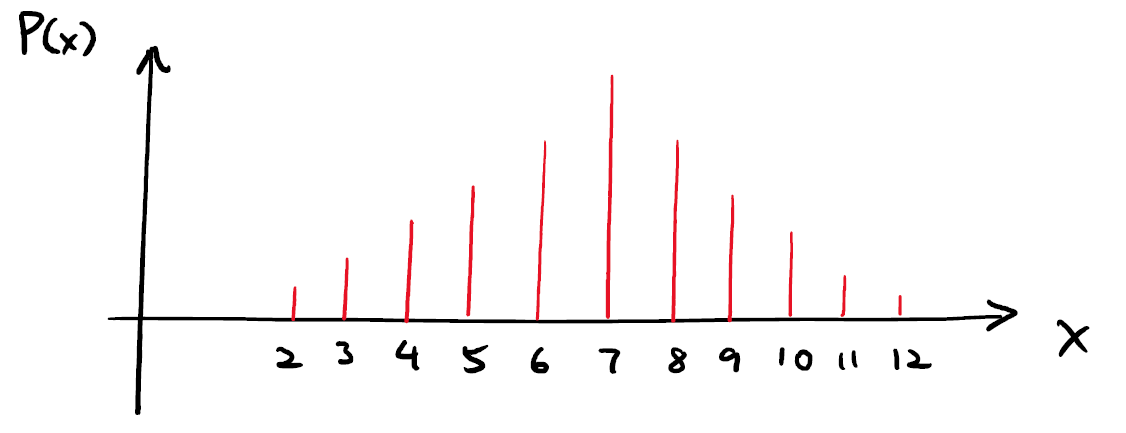
\includegraphics[width=\textwidth]{pmf}
    \end{minipage}
\end{center}

\begin{itemize}
    \item \bf{\ul{Normalization requriement}}:
    The probabilities of all possible outcomes add up to 1.
    \aleq{
        \sum_{\text{all possible }x_i} P(x_i) = 1
    }

    \item \bf{\ul{Expected value}}: 
    i.e. The weighted average of all outcomes according to the probabilities,
    which is the average value you would get after repeating the process $\infty$ times.
    \aleq{
        \E[x]\quad \defeq \sum_{\text{all possible }x_i} x_i P(x_i)
    }

    \item \bf{\ul{Variance}}:
    It is the average of $(\text{distance})^2$ of all outcomes relative to the expected value.
    Taking square root gives the \bf{standard derivation} (S.D.) = $\sqrt{\text{Variance}}$. 
    \addBentArrow[red]{En}{(-4ex,-2ex)}{\scriptsize Then take average}
    {(0,-1.5ex)}{(-6ex,0.5ex)}
    \addBentArrow[blue]{var}{(4ex,-2ex)}
    {\scriptsize $(x-\E{x})$ = x's distance from the expected value\\[-1ex] \scriptsize Square for taking magnitude only}
    {(0,-1.5ex)}{(17.5ex,-0.5ex)}
    \aleq{
        \Var{x} &\defeq 
        \tkn{En}{\cul[red]{\E}}[\tkn{var}{\cul[blue]{(x-\E{x})^2}}]
    }
    
\end{itemize}

\begin{notation}[Side note:]
    In a special case where there are $N$ different outcomes and every outcome has equal probability to occur,
    \aleq{
        P(x_i) = \frac{1}{N}
    }
    Then the expected value, variance and S.D. will reduce to the mean and S.D. formula that we can find in high school textbook.
    \aleq{
        \E{x} &= \sum_{\text{all possible }x_i} x_i P(x_i) = \frac{\sum_i x_i}{N} \ \defeq\ \bar{x} \\[1ex]
        %
        \Var{x} &= \E{(x-\E{x})^2} = \frac{\sum_i (x_i-\E{x})^2}{N} = \frac{\sum_i (x_i-\bar{x})^2}{N} \\[1ex]
        %
        \text{S.D.} = \sqrt{\Var{x}} &= \sqrt{\frac{\sum_i (x_i-\bar{x})^2}{N}}
    }

\end{notation}


%%%%%%%%%%%%%%
\subsection{Probability Density Function (PDF)}

For random variables that can apprear as any value within an interval,
we describe them using the \bf{probability density function} (PDF).

\begin{center}
    \begin{minipage}{0.5\linewidth}
        \centering
        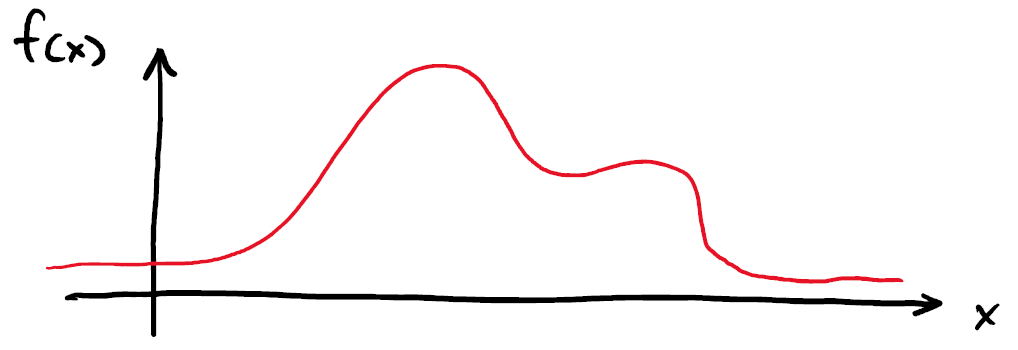
\includegraphics[width=\textwidth]{pdf}
    \end{minipage}
\end{center}


Pay attention here: the output value of the PDF, $f(x)$, 
is NOT the probability of getting $x$. 
This is because there are always infinitely many real number along any interval of real numbers.
\red{The probability of getting an exact number is limited to $0$.}\\

Instead, PDF can only describe the probability of getting a value within an interval $[x_0,x_0+\dd{x}]$.
\aleq{
    P(\tkn{pdf_range}{\cul[green]{x_0<x<x_0+\dd{x}}}) = \tkn{pdf_f}{\cul[blue]{f(x)}}\tkn{pdf_dx}{\cul[red]{\dd{x}}}
}
\addArrow[green]{pdf_range}{(0,-2ex)}{\scriptsize Prob. inside the interval}{(0,-1ex)}
\addArrow[blue]{pdf_f}{(0,-3ex)}{\scriptsize height}{(0,-1.5ex)}
\addArrow[red]{pdf_dx}{(3ex,-2ex)}{\scriptsize width}{(0,-1ex)}


\begin{center}
    \begin{minipage}{0.6\linewidth}
        \centering
        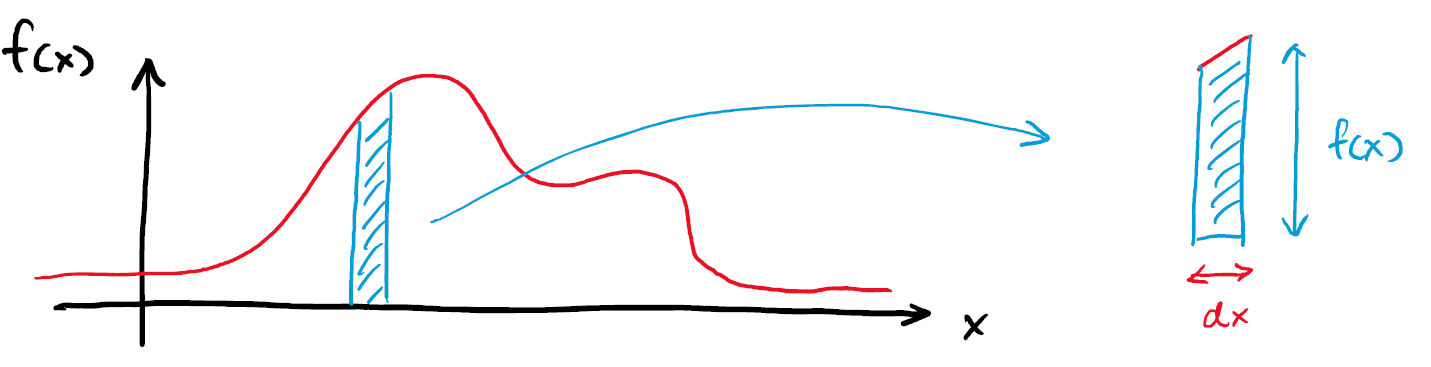
\includegraphics[width=\textwidth]{pdf_area}
    \end{minipage}
\end{center}

As interpreted, the probability is represented by the \cul[red]{area under curve $f(x)\dd{x}$},
not the height $f(x)$. This is also why it is named "density" function - 
the probability per "length" of $x$.

\newpage
The formula for PMF (discrete cases) can be extended to PDF (continuous cases).
\begin{itemize}
    \item \bf{\ul{Normalization requriement}}: 
    The probabilities of all possible cases add up to 1.
    From the condition for PMF, we can extend the sum to integral for PDF.
    \aleq{
        \sum_{\text{all possible }x_i} P(x_i) = 1 
        \qquad\Rightarrow\qquad 
        \int_{-\infty}^\infty f(x) \dd{x} = 1
    }

    \item \bf{\ul{Expected value}}: 
    The weighted average of all outcomes according to the probabilities.
    Can be understand by the weighted sum interpretation of integration.
    \aleq{
        \E{x}\quad \defeq \sum_{\text{all possible }x_i} x_i P(x_i) 
        \qquad\Rightarrow\qquad
        \E{x} \ \defeq\  \int_{-\infty}^{\infty} xf(x) \dd{x}
    }

    \item \bf{\ul{Variance}}:
    Same as in the discrete case, it is the average of $(\text{distance})^2$ of all outcomes relative to the expected value.
    \aleq{
        \Var{x}\ \defeq\ \E{(x-\E{x})^2} 
        \qquad\Rightarrow\qquad
        \Var{x} \ \defeq\  \int_{-\infty}^{\infty} (x-\E{x})^2 f(x) \dd{x}
    }
    Taking square root gives the standard derivation (S.D.) = $\sqrt{\Var{x}}$. 

\end{itemize}


\linesep
% Section %%%%%%%%%%%%%%%%%%%%%%%%%%%%%%%%%%%%%%%%%%%%%%%%%%%%
\section{Fluctuation \& Equilibrium}

%%%%%%%%%%%%%%%%%
\subsection{Fluctuation of State Parameters}

From previous notes, we have learnt that 
\begin{itemize}
    \item Different states of a thermodynamics system are distinguished by macrostate parameters.
    \item Change of macrostate is caused by random motion. 
    \item Every \it{closed} system will eventually evolve into a state with maximum multiplicity, 
    because the probability to observe a macrostate is proportional to its multiplicity.
\end{itemize}

In general, if we can express the entropy $S$ of system in terms of a macrostate parameter $x$,
We can compute the corresponding $x=x_0$ at the maximum entropy state by solving
    \aleq{
        \begin{cases}
            \eval{\dvv{S}{x}}_{x=x_0} = 0 
            & \qty(\substack{\text{Entropy is at its maximum}\\\Rightarrow \text{ Slope }=\, 0 \text{ at }x=x_0})\\[1em]
            %
            \eval{\dvv[2]{S}{x}}_{x=x_0} <0
            & \qty(\substack{\text{Slope keeps decreasing}\\\text{near the maximum}})
        \end{cases}
    }

However, because of random motion, 
even if the system has reached its maximum entropy state,
its state parameters can still fluctuate.
Every so often, the parameter $x$ may deviate by some small amount $\Delta x$, 
causing the system entering a lower entropy state. 
But this change will revert very soon again due to random motion.\\

For example, in the 2-boxes system with 1000 balls, 
its macrostates can be distinguished by one state parameter - 
$N_R=$ the number of balls in the right box. 
Because the balls are free to move (randomly) between the boxes, 
$N_R$ must fluctuate, even when it has reached the maximum entropy state 500L-500R. 
\begin{itemize}
    \item
    One of the ball may temporarily move from the left box to the right box.
    The system's state change to 499L-501R. 

    \item After some time, another ball moves from the right box to the left box.
    The system's state returns to 500L-500R.
\end{itemize}

\insertFig{moving ball in and out}


In fact, we can determine the probability distribution of observing fluctuation $\Delta x$.
Recall that the probability of observing a macrostate with parameter $x$ 
is proportional to the number of microstates (i.e. multiplicity) it corresponds to,
\aleq{
    P\qty(x=x_0) \ &\propto\ 
    \qty(\mstack{\text{\# of microstates that}\\\text{leads to observing }x=x_0})\\[1em]
    &= \frac{W(x=x_0)}{Z} = \frac{e^{\frac{S(x=x_0)}{k}}}{Z}
}

where $Z$ is just some constant for normalization (because probability should add up to $1$).
\aleq{
    Z = 
    \begin{cases}
        \displaystyle \sum_{\substack{\text{all possible}\\x_i}}W(x_i) 
        = \sum_{\substack{\text{all possible}\\x_i}}e^{\frac{S(x_i)}{k}}
        & \text{if }x \text{ must take discrete values}\\[2.5em]
        %
        \displaystyle \int_{\substack{\text{possible}\\\text{range of }x}} W(x) \dd{x} 
        = \int_{-\infty}^\infty e^{\frac{S(x)}{k}} \dd{x} 
        & \text{if }x \text{ can take continuous values}
    \end{cases}
}

Let $x=x_0$ when the system is at its maximum entropy state,
the fluctuation in entropy $\Delta S$ can be related to 
the fluctuation of the state parameter $\Delta x$ by Taylor series expansion:
\aleq{
    S(x_0+\Delta x) &= S(x_0) + \Delta S\\ 
    %
    &= \cub[green]{S(x_0)}{\text{A constant}} + \cub[red]{\ccancelto[red]{0}{\dvv{S}{x}\eval_{x=x_0}}}{\substack{S\, =\, \text{max.}\\\text{so slope }=\,0}} (\Delta x) 
        + \half \cub[blue]{\dvv[2]{S}{x}\eval_{x=x_0}}{\substack{S\,=\,\text{max.}\\\text{\nth{2} derivative }<\,0}} (\Delta x)^2 + \cdots
}

The probability distribution of $x=x_0+\Delta x$ is therefore approximately
\aleq{
    P\qty(x) &=
    \frac{e^{\frac{S(x)}{k}}}{Z} \\
    %
    &\approx \cub[green]{\inv{Z} \cdot e^{\frac{S(x_0)}{k}}}{\substack{\text{Both are constant}\\\text{can combine}}} 
    \cdot e^{\inv{2k}\dv[2]{S}{x}\eval_{x_0}(\Delta x)^2}\\[1ex]
    %
    &= \inv{Z'} \cdot e^{\inv{2k}\dv[2]{S}{x}\eval_{x_0}(x-x_0)^2}
}

This probability is in the form of \bf{normal distribution} (also called Gaussian distribution),
whose standard formula is written as
\aleq{
    P(x) = \inv{\sqrt{2\pi\sigma^2}} \cdot e^{-\frac{(x-\mu)^2}{2\sigma^2}}
}
A normal distribution is governed by two variables, $\mu$ and $\sigma$, 
which are the mean and standard derivation of the distribution respectively.

\insertFig{gaussian distribution}

By comparison, we can identify that the distribution of $x$ follows a normal distribution with
\begin{itemize}
    \item \ul{Mean}: $\mu=x_0$\\
    As expected, $x$ should fluctuate around $x=x_0$,
    which is the value of $x$ when the system is in the maximum entropy state.
    
    \item \ul{Standard derivation}: $\sigma = -\qty(\inv{k}\dv[2]{S}{x}\eval_{x_0})^{-\half}$\\
    i.e. The size of fluctuation depends on the \nth{2} derivative of $S$ with respect to $x$.

\end{itemize}


\begin{notation}[Side note:]
    Recall in Clausius theorem - 
    entropy of a closed system must either be a constant 
    or increase along any process.
    But because macrostate parameters are always fluctuating due to random process,
    entropy can fluctuate too. 
    Clausius theorem should be more accurately written as:
    \aleq{
        \Delta S \geq 0 \quad\xRightarrow{\text{More accurately}}\quad \Delta S_\red{\text{avg.}} \geq 0
    }

\end{notation}




%%%%%%%%%%%%%%
\subsection{Thermal Equilibrium}

In a closed system, the total energy must conserve within the system.
However because thermal fluctuation is allowed,
the internal energy of individual objects in the system are not constants
but fluctuate around some values.

\insertFig{2 object exchange heat}

For simplicity, we can consider a system with only 2 objects $A$ and $B$.
Because the total energy $U_\text{total}$ is conserved, 
if $A$ has an internal energy $U_A$, $B$ must have an internal energy $U_B = U_\text{total}- U_A$.
\begin{center}
    \blue{Solely using $U_A$ is enough to distinguish different states.\\
    We can investigate the fluctuation of $U_A$ as a state parameter.}
\end{center}

Suppose the two objects' entropy can be expressed in terms of their internal energy: 
\aleq{
    S_A = S_A(U) \quad\text{and}\quad S_B = S_B(U)
}
We can determine at what condition when the system is at the maximum entropy state.  
Because entropy of a system is the sum of entropy of individual objects,
\aleq{
    S_\text{total} = S_A(U_A) + S_B(U_B) = S_A(U_A) + S_B(U_\text{total} - U_A)
}

At the maximum entropy state, $\dvv{U_A}S_\text{total} = 0$.
\aleq{
    \dvv{U_A} S_\text{total} 
    &= \dvv{S_A}{U_A} + \dvv{S_B}{U_A} \\[1ex]
    &= \dvv{S_A}{U_A} + \dvv{S_B}{U_B} \cdot \dvv{U_A}(U_\text{total} - U_A)\\[1ex]
    &= \dvv{S_A}{U_A} - \dvv{S_B}{U_B}\\[1ex]
    &=0\\[1ex]
    \gray{\inv{T_A} \ \defeq\ \, }\dvv{S_A}{U_A} &= \dvv{S_B}{U_B} \gray{\ \, \defeq\ \inv{T_B}}
}

\vskip 1ex
This result implies - If the objects' entropy-energy relation $S(U)$ is known,
we can define a state parameter $T=\dvv{U}{S}$ (so-called "temperature"), 
which can be used to indicate \bf{thermal equilibrium}: 
\begin{center}
    \begin{minipage}{0.8\textwidth}
        \begin{framed}
            \centering
            Thermal equilibrium occurs at the maximum entropy state of a system, 
            when every object's "$T$" parameter must be equal.
        \end{framed}
    \end{minipage}
\end{center}

Remember: Thermal equilibrium only requires objects to have equal temperature.
Fluctuation in internal energy is still allowed.
Since the \nth{2} derivative of $S$ by $U_A$ is 
\aleq{
    \dvv[2]{S}{U_A} = \dvv{U_A}\qty(\inv{T}) = -\inv{T^2}\dvv{T}{U_A} = -\inv{T^2C_V}
}
where $C_V$ is the heat capacity of object $A$ under constant volume process.
So the distribution of $U_A$ is a normal distribution:
\begin{itemize}
    \item Centered around some equilibrium value $U_{0}$.\\
    (we cannot solve the value without knowing what exactly are $S_A(U)$ and $S_B(U)$.)

    \item Standard derivation $= T\sqrt{kC_V}$.\\
    This is the characteristic size of energy fluctuation of a system.
\end{itemize}

\insertFig{normal distribution with standard derivation: 95\% lies within 2SD}

How large is this energy fluctuation?
Asumming room temperature $T\sim 300$K,
\begin{itemize}
    \item In daily life scale: 
    \begin{itemize}
        \item Heat capacity of materials $C_V\sim 10^3$J/K. 
        \item Energy fluctuation on objects is therefore of magnitude $\sim 10^{-10}$J
    \end{itemize}
    which is completely negligible in our daily life.

    \item In atomic scale:
    \begin{itemize}
        \item One ideal gas particle has a heat capacity $C_V= \frac{3}{2}k$.
        \item Energy fluctuation on one particle is therefore $T\sqrt{kC_V} \sim kT \sim 10^{-21}$J.
        \item Mass of a proton/neutron is in the scale $m\sim 10^{-27}$kg.
    \end{itemize}
    A sudden fluctuation in energy is enough to accelerate a particle's speed by $\sim 1000$m/s!
    \aleq{
        \Delta U = kT \approx \half m(\Delta v)^2 \sim 10^{-21} \qquad\Rightarrow\qquad \Delta v = \sqrt{\frac{kT}{m}} \sim 10^3
    }
\end{itemize}
 
This tells us what actually happens in thermal equilibrium:
\begin{center}
    \begin{minipage}{0.9\textwidth}
        \begin{framed}
            \centering
            The concept of thermal equilibrium is "sensible" only for objects in large scale,\\
            so that any effects of energy fluctuation are averaged out by random motion.\\
            But in microscopic scale, the particles are interacting violently all the time.
        \end{framed}
    \end{minipage}
\end{center}

\insertFig{normal scale: quiet; microscale: crazy}


%%%%%%%%%%%%
\subsection{Boltzmann Factor}

Because of the scale of energy fluctuation is so big for a particle,
we cannot expect the internal energy of a particle to always stay around the value which maximize the entropy of the object.
(It is the \cul[red]{average} $U$ that maximizes the entropy, not the $U$ on a single particle.)
\begin{center}
    \red{What is the probability for a particle having a specific energy $U$ under thermal equilibrium?}
\end{center}

We can model by isolating a particle with the rest of every particle in a box. 
Although the particle may be moving crazily due to thermal fluctuation, 
we know that the rest of the particles are "collectively" forming a thermal equilibrium of temperature $T$.

\insertFig{heat bath model: bath = rest of particle, temp T; obj = 1 particle, no T defined}

Let the total energy to be a constant $U_\text{total}$.
Obviously, the energy carried by 1 particle $U_p$ should be way less than that carried by the rest $U_\text{rest}$.
We can write
\aleq{
    U_\text{total} = U_\text{rest} + U_p = \text{const.} 
    \qquad\text{and}\qquad 
    U_\text{rest} \gg U_p
}

Let the entropy of the rest of the particle be some function $S_\text{rest} = S_\text{rest}(U_\text{rest})$.
We can make a Taylor expansion by
\aleq{
    S_\text{rest} &= S_\text{rest}(U_\text{rest}) \\
    %
    &= S_\text{rest}(U_\text{total} - U_p)\\[1ex]
    %
    &\approx S_\text{rest}(U_\text{total}) - \dvv{S_\text{rest}}{U}\eval_{U=U_\text{total}}\cdot U_p\\
    %
    &\approx S_\text{rest}(U_\text{total}) - \frac{U_p}{T}
}

The total multiplicity of the box is thus
\aleq{
    S_\text{total} &= S_\text{rest}+ S_p\\
    %
    W_\text{total} &= e^\frac{S_\text{rest}+ S_p}{k} \\
    %
    &\approx e^\frac{S_\text{rest}(U_\text{total}) -  \frac{U_p}{T}}{k} \cdot e^\frac{S_p}{k}\\
    %
    &= e^\frac{S_\text{rest}(U_\text{total})}{k} \cdot e^{-\frac{U_p}{kT}} \cdot e^\frac{S_p}{k}\\
    %
    &= \tkn{W_const}{\cul[red]{e^\frac{S_\text{bath}(U_\text{total})}{k}}} \cdot e^{-\frac{U_p}{kT}} \cdot \tkn{W_obj}{\cul[blue]{W_p(U_p)}}
}
\addArrow[red]{W_const}{(-3ex,-2ex)}
{\scriptsize $U_\text{total}$ is a constant\\[-1ex]\scriptsize so this term is just a constant}
{(0,-1ex)}{(-3ex,-1.5ex)}
\addArrow[blue]{W_obj}{(3ex,-2ex)}
{\scriptsize Multiplicity of the particle\\[-1ex]\scriptsize is some function of $U_p$}
{(0,-1.5ex)}{(5ex,-1.5ex)}

\vskip 1em
Now the total multiplicity is a function of $U_p$ only.
Thus we can calculate the probability that the particle acquire an internal energy $U_p$:
\aleq{
    P\qty(U=U_p) \ &\propto\ 
    \qty(\mstack{\text{\# of microstates that}\\\text{leads to observing }U=U_p})\\[1ex]
    %
    &= W_\text{total}(U_p)\\[1ex]
    %
    &\propto e^{-\frac{U_p}{kT}}\cdot W_p(U_p)
}

\vskip 1ex
Upon normalizing, we define the \bf{Boltzmann distribution} - 
the probability of finding a particle with internal energy $U$ within an object/system 
that is in thermal equilibrium of temperature $T$.
\aleq{
    \Aboxed{
        P\qty(U) &= \frac{e^{-\frac{U}{kT}}\cdot W_p(U)}{Z}
    }
}

The components of the Boltzmann distribution also have some fancy names:
\begin{itemize}
    \item The term $e^{-\frac{U}{kT}}$ is called the \bf{Boltzmann factor}.
    
    \item The normalization constant $Z$ is called \bf{partition function}, which calculates as
    
    \aleq{
        Z = 
        \begin{cases}
            \displaystyle \sum_{\substack{\text{all possible}\\\text{values of }U}}e^{-\frac{U}{kT}}\cdot W_p(U) 
            & \text{if }U \text{ must take discrete values}\\[2.5em]
            %
            \displaystyle \int_{\substack{\text{possible}\\\text{range of }U}} e^{-\frac{U}{kT}}\cdot W_p(U) \dd{U} 
            & \text{if }U \text{ can take continuous values}
        \end{cases}
    }

\end{itemize}


\begin{example}
    Suppose now the fluctuation is not on one particle, but four particles - 
    which these four particles is contained in a 2-boxes system, 
    and particles in the right box would have higher potential energy than in the left box by $\epsilon$.

    \insertFig{bath model -> connect to 2 boxes model -> show energy diagram}

    Given that the thermal equilibrium side is at temperature $T$.
    What is the probability to find each of the macrostate of 2-boxes system?
    First we can tabulate the macrostates and their multiplicity:\\

    where the normalization constant (partition function) is just the sum of all the multiplicity:
    \aleq{
        Z = e^0\cdot 1 + e^{-\frac{\epsilon}{kT}}\cdot 4 + e^{-\frac{2\epsilon}{kT}}\cdot 6
            + e^{-\frac{3\epsilon}{kT}}\cdot 4 + e^{-\frac{4\epsilon}{kT}}\cdot 1
    }

\end{example}    

\linesep
% Section %%%%%%%%%%%%%%%%%%%%%%%%%%%%%%%%%%%%%%%%%%%%%%%%%%%%
\section{Speed Distribution of Ideal Gas}

Because the energy of an ideal gas particle can be chosen from a continuous range of value,
we should use the continuous version of Boltzmann distribution:
writing the probability of a particle acquiring an energy in the range $[U_0,U_0+\dd{U}]$ as
\aleq{
    P\qty(U_0<U<U_0+\dd{U}) = f(U_0)\dd{U} = \frac{e^{-\frac{U_0}{kT}}\cdot W_p(U_0)}{Z}\dd{U}
}

What is the function of multiplicity, $W_p(U)\dd{U}$, for ideal gas particles?



%%%%%%%%%%%%%%
\subsection{Multiplicity of Ideal Gas}

In the mechanics picture,
microstates of a particle are described by its position and velocity:
\aleq{
    \text{microstate} = (\vvec{r}, \vvec{v}) = (x,y,z, v_x, v_y, v_z)
}

Suppose the gas particle is in a container of size $L\times L \times L$ and 
there is no potential energy difference anywhere.
The possibilities of the 6 state parameters are
\begin{itemize}
    \item $x,y,z$ = Equal probability to be any real number within $[0,L]$.
    
    \item $v_x,v_y,v_z$ = Equal probability to be any real number as long as $\sqrt{v_x^2+v_y^2+v_z^2}<(\text{speed of light})$
    
\end{itemize} 

To visualize, the possible states can be plotted in a 6-dimension state space of $(x,y,z, v_x, v_y, v_z)$ 

\insertFig{3D x3D space; xyz form cube; v form sphere}


Because there is no potential energy difference anywhere in the box,
we can choose the potential energy of the particle to be $0$.
So the particle's internal energy is equal to its kinetic energy, which is a function of the velocities only.
\aleq{
    U = \text{K.E.} + \text{P.E.} = \half m(v_x^2+v_y^2+v_z^2) + 0
}

So what is the multiplicity of a marcostate with internal energy in the range $[U_0,U_0+\dd{U}]$?
It is the number of microstates $(x,y,z, v_x,v_y,v_z)$ that satisfy $U_0\leq \half m(v_x^2+v_y^2+v_z^2)\leq U_0+\dd{U}$.

\insertFig{xyz every point satisfy anyway, v form sphere}

In the $x$-$y$-$z$ space, every point is allowed. 

In the $v_x$-$v_y$-$v_z$ space, 
only the points with $\norm{\vvec{v}} = \sqrt{v_x^2+v_y^2+v_z^2}$ in between $\qty[\sqrt{\frac{2U_0}{m}}, \sqrt{\frac{2(U_0+\dd{U})}{m}}]$ are allowed.\\

\begin{itemize}
    \item Because multiplicity due to different $(x,y,z)$ is the the same for any value of $U$,
    it shall be canceled by normalization when we compute probability.
    We can ignore it from now on.

    \item For the multiplicity due to different $(v_x,v_y,v_z)$,
    although technically there are infinitely many points inside the spherical shell,
    this number of points must be proportional to the volume of the spherical shell.
    \aleq{
        (\text{Volume of the shell}) = 4\pi \norm{\vvec{v}}^2 \dd{\norm{\vvec{v}}}
        \quad\Rightarrow\quad
        (\text{\# of points within})\propto 4\pi \norm{\vvec{v}}^2 \dd{\norm{\vvec{v}}}
    }
    Again, because any proportionality constant should be the same for any value of $U$, 
    it shall be canceled by normalization when we compute probability.

\end{itemize}

By change of variable $\norm{\vvec{v}} = \sqrt{\frac{2U}{m}}$ and $\dd{\norm{\vvec{v}}} = \sqrt{\inv{2mU}}\dd{U}$,
we get $W(U)\dd{U}$:
\aleq{
    W(U_0)\dd{U} &= \qty(\mstack{\text{\# of microstates that satisfy}\\U \in [U_0,U_0+\dd{U}]})\\[1ex]
    %
    &= \qty(\mstack{\text{\# of microstates that satisfy}\\\textstyle \norm{\vvec{v}} \in \qty[\sqrt{\frac{2U_0}{m}}, \sqrt{\frac{2(U_0+\dd{U})}{m}}]})\\[1ex]
    %
    &\cul[red]{\propto}\ \qty(\mstack{\text{Volume of spherical shell in between radius}\\\textstyle \sqrt{\frac{2U_0}{m}}\leq \norm{\vvec{v}}\leq \sqrt{\frac{2(U_0+\dd{U})}{m}}})\\[1ex]
    %
    &= 4\pi \norm{\vvec{v}}^2 \dd{\norm{\vvec{v}}}\\[1ex]
    %
    &= 4\pi\qty(\frac{2U_0}{m})\sqrt{\inv{2mU_0}}\dd{U}\\[1ex]
    %
    &= 4\pi\sqrt{\frac{2}{m^3}}\sqrt{U_0}\dd{U}
}

\begin{notation}[Side note:]
    Note that because of the \cul[red]{proportionality symbol} above,
    the $W(U)$ we arrived at is NOT the number of state of ideal gas,
    but the \bf{density of state} - the number of state per unit volume in the $v_x$-$v_y$-$v_z$ space.\\

    Calculating the exact number of state requires quantum mechanics.
    Because at the smallest scale, 
    quantum mechanics tells us that internal energy of particles can only take quantized values.
    Then we can actually count the number of allowed states.
\end{notation}


%%%%%%%%%%%%%%
\subsection{Normalization: Gaussian Integral}

Now we can write down the Boltzmann distribution of ideal gas:
\aleq{
    P(U)\sim f(U)\dd{U} = \frac{e^{-\frac{U}{kT}}\cdot W_p(U)}{Z} 
    = \frac{\ccancelto[red]{\text{constant}}{4\pi\sqrt{\frac{2}{m^3}}}\cdot  e^{-\frac{U}{kT}}\sqrt{U}\dd{U}}{\ccancelto[red]{}{Z}}
    = \frac{e^{-\frac{U}{kT}}\sqrt{U}\dd{U}}{Z}
}

The remaining is to calculate the normalization constant $Z$. 
Let $x^2 = \frac{U}{kT}$ and $2x\dd{x} = \inv{kT}\dd{U}$,
\aleq{
    \tkn{half_range}{\cul[red]{\int_0^\infty}} f(U) \dd{U} 
    &= \inv{Z}\int_0^\infty e^{-\frac{U}{kT}}\sqrt{U}\dd{U}\\[1ex]
    %
    &= \inv{Z}\int_0^\infty e^{-x^2}\sqrt{x^2kT} \cdot (kT)\cdot 2x\dd{x}\\[1ex]
    %
    &= \frac{2(kT)^{\frac{3}{2}}}{Z} \int_0^\infty e^{-x^2}x^2\dd{x}\\[1ex]
    %
    &\equiv 1 \quad(\text{Required by normalization})
}
\addBentArrow[red]{half_range}{(-4ex,-2ex)}
{\scriptsize $U$ of ideal gas = K.E.\\[-1ex]\scriptsize can only take positive values}{(0,-3ex)}{(-8ex,0)}

This integral is extremely tricky to compute.
First we do integration by-part,
\aleq{
    \int_0^\infty e^{-x^2}x^2\dd{x} 
    &= \int_0^\infty \half e^{-x^2}x\dd{x^2} \\[1ex]
    %
    &= -\int_0^\infty \half x \dd{e^{-x^2}} \\[1ex]
    %
    &= \ccancelto[red]{0}{-\eval{\qty(\half xe^{-x^2})}_0^\infty} + \half \int_0^\infty e^{-x^2} \dd{x}\\[1ex]
    %
    &= \half \int_0^\infty e^{-x^2} \dd{x}
}

The integral on $e^{-x^2}$ is called the \bf{Gaussian integral},
which can be analytically computed only if the bounds are $\pm \infty$.
\aleq{
    \Aboxed{
        \int_{-\infty}^\infty e^{-x^2} \dd{x} \equiv \sqrt{\pi}
    }
}

But the range in our integral is only $[0,\infty]$, not $[-\infty, \infty]$,
we only take half of it (because $e^{-x^2}$ is an even function, $f(x)=f(-x)$).
So the normalization constant $Z$ is 
\aleq{
    Z &= 2(kT)^{\frac{3}{2}}\int_0^\infty e^{-x^2}x^2\dd{x}\\[1ex]
    &= 2(kT)^{\frac{3}{2}}\cdot \half\cdot \frac{\sqrt{\pi}}{2}\\[1ex]
    &= \frac{\sqrt{\pi k^3T^3}}{2}
}

The complete expression of Boltzmann distribution for ideal gas is therefore
\aleq{
    \Aboxed{
        f(U)\dd{U} = \frac{2}{\sqrt{\pi k^3T^3}}e^{-\frac{U}{kT}}\sqrt{U}\dd{U}
    }
}


\begin{notation}[Side note:]
    The standard method of computing Gaussian integral is as follow:
    \begin{enumerate}
        \item Let $\displaystyle I = \int_{-\infty}^{\infty} e^{-\half ax^2} \dd{x}$. 
        The trick of computation is to promote it to 2D:
        \aleq{
            I^2 &= \qty(\int_{-\infty}^{\infty} e^{-\half ax^2} \dd{x} )
                \cdot \qty(\int_{-\infty}^{\infty} e^{-\half ay^2} \dd{y}) \\[1em]
            %
            &= \int_{x=-\infty}^{x=\infty}\int_{y=-\infty}^{y=\infty} 
                e^{-\half ax^2} e^{-\half ay^2} \dd{y} \dd{x} \\[1em]
            %
            &= \int_{x=-\infty}^{x=\infty}\int_{y=-\infty}^{y=\infty} 
                e^{-\half a(x^2+y^2)} \dd{y} \dd{x} 
        }

        \item The we can do a change of coordinate from $x$-$y$ to polar $r$-$\theta$: 
        \aleq{
            \iint f(x,y)\dd{x}\dd{y} \quad\Leftrightarrow\quad \iint f(r,\theta)\, r\dd{r}\dd{\theta}
        }
        \begin{itemize}
            \item Converting the integrand:
            \aleq{
                e^{-\half a(x^2+y^2)} \quad\Leftrightarrow e^{-\half ar^2}
            }
            

            \item The integration range is always the whole 2D plane:
            \aleq{
                (x,y) \in \{-\infty,\infty\}\times \{-\infty,\infty\} 
                \quad \Leftrightarrow\quad
                (r,\theta) \in \{0,\infty\}\times  \{0,2\pi\}
            }
        \end{itemize}

        \item So the integral becomes 
        \aleq{
            I^2 &= \int_{r=0}^{r=\infty} \int_{\theta=0}^{\theta=2\pi} e^{-\half ar^2}r\dd{\theta}\dd{r}\\
            %
            &= 2\pi \cdot \int_{r=0}^{r=\infty} e^{-\half ar^2} \dd{\qty(\frac{r^2}{2})}\\
            %
            &= \frac{2\pi}{a}\\
            %
            I &= \sqrt{\frac{2\pi}{a}}
        }
            
    \end{enumerate}
\end{notation}


%%%%%%%%%%%%%%
\subsection{Speed Distribution \& Average Speed}

The final derivation is the famous Maxwell-Boltzmann distribution,
which plots the probability of finding ideal gas particles at different speed $v$.
The derivation is straightforward,
by substituting $U = \half mv^2$ and $\dd{U}=mv\dd{v}$ into the Boltzmann distribution.
\aleq{
    f(U)\dd{U} &= \frac{2}{\sqrt{\pi k^3T^3}}e^{-\frac{U}{kT}}\sqrt{U}\dd{U}\\
    %
    &= \frac{2}{\sqrt{\pi k^3T^3}}e^{-\frac{mv^2}{2kT}}\sqrt{\half mv^2} \cdot mv\dd{v}\\
    %
    \Aboxed{
        f(v)\dd{v} &= \sqrt{\frac{2m^3}{\pi k^3T^3}} v^2e^{-\frac{mv^2}{2kT}} \dd{v}
    }
}


In physics textbooks you can find 2 different formulas related to the average speed of ideal gas. 
these are derived as the expected values over the Maxwell-Boltzmann distribution.

\begin{enumerate}
    \item \bf{\ul{Average Speed}} = Expected value to $v$, i.e. $\E{v}$.
    \aleq{
        \E{v} &= \int^\infty_0 v \cdot f(v) \dd{v}\\[1ex]
        %
        &= \int^\infty_0 v \cdot \sqrt{\frac{2m^3}{\pi k^2 T^3}} v^2 e^{-\frac{mv^2}{2kT}} \dd{v}\\[1ex]
        %
        &= \sqrt{\frac{2m^3}{\pi k^2 T^3}} \qty(\frac{2kT}{m})^2 
        \int^\infty_0 \tkn{x1}{\cul[blue]{\qty(\sqrt{\frac{m}{2kT}}v)^3 e^{-\qty(\sqrt{\frac{m}{2kT}}v)^2} \dd{\qty(\sqrt{\frac{m}{2kT}}v)}}}\\[1ex]
        %
        &= \sqrt{\frac{32kT}{\pi m}} \tkn{int1}{\cul[red]{\int^\infty_0 x^3 e^{-x^2} \dd{x}}} \\[1ex]
        %
        &= \sqrt{\frac{32kT}{\pi m}} \cdot \half\\[1ex]
        %
        \Aboxed{
            v_\text{avg}\ \defeq\ \E{v} &= \sqrt{\frac{8kT}{\pi m}}
        }
    }
    \addArrow[blue]{x1}{(0,-3ex)}{\scriptsize Let $x=\sqrt{\frac{m}{2kT}}v$}{(0,-3.2ex)}{(0,-0.8ex)}
    \addBentArrow[red]{int1}{(5ex,-2ex)}
    {\scriptsize This integral can be computed\\[-1ex]\scriptsize by substitution and by-part\\[-1ex]\scriptsize No need to use Gaussian integral}{(0,-3ex)}{(11.5ex,-0.5ex)}

    \item \bf{\ul{Root Mean Square Speed}} = $\sqrt{\text{Expected value to } v^2}$, i.e. $\sqrt{\E{v^2}}$.
    \aleq{
        \E{v^2} 
        &= \int^\infty_0 v^2 \cdot f(v) \dd{v}\\[1ex]
        %
        &= \int^\infty_0 v^2 \cdot \sqrt{\frac{2m^3}{\pi k^2 T^3}} v^2 e^{-\frac{mv^2}{2kT}} \dd{v}\\[1ex]
        %
        &= \sqrt{\frac{2m^3}{\pi k^2 T^3}} \qty(\frac{2kT}{m})^3 
        \int^\infty_0 \tkn{x2}{\cul[blue]{\qty(\sqrt{\frac{m}{2kT}}v)^3 e^{-\qty(\sqrt{\frac{m}{2kT}}v)^2} \dd{\qty(\sqrt{\frac{m}{2kT}}v)}}}\\[1ex]
        %
        &= \sqrt{\frac{64k^2T^2}{\pi m^2}} \tkn{int2}{\cul[red]{\int^\infty_0 x^4 e^{-x^2} \dd{x}}} \\[1ex]
        %
        &= \sqrt{\frac{64k^2T^2}{\pi m^2}}\cdot \frac{3\sqrt{\pi}}{8} \\[1ex]
        %
        &= \frac{3kT}{m}\\[1ex]
        %
        \Aboxed{
            v_\text{rms} \ \defeq\  \sqrt{\E{v^2}} &= \sqrt{\frac{3kT}{m}}
        }
    }
    \addArrow[blue]{x2}{(0,-3ex)}{\scriptsize Let $x=\sqrt{\frac{m}{2kT}}v$}{(0,-3.2ex)}{(0,-0.8ex)}
    \addBentArrow[red]{int2}{(5ex,-2ex)}
    {\scriptsize This requires computing\\[-1ex] \scriptsize Gaussian integral}{(0,-3ex)}{(8ex,0)}

\end{enumerate}

Because the average KE (which is something we can measure) is calculated as 
\aleq{
    \text{Avg. KE} &= \E{\qty(\half m\abs{v}^2)} \\
    &= \half m \E{\abs{v}^2}\\
    &= \half m v_\text{rms}^2 
    = \frac{3}{2}kT
}

The root mean square speed is used much more commonly than the average speed.

%%%
\theend
\end{document}